\chapter{理论技术与公式化表达}
本章将详细从基础理论知识与应用方式介绍联邦学习、深度神经网络以及子模型全局优化三个重要的知识。
上述的技术是理解后续论文的重要基础,构成了本文的研究核心部分,对于学习全文具有重要的意义。

\section{联邦学习公式化与优化目标}
联邦学习\cite{mcmahan2017communication}是由谷歌在2017年提出的一种创新性的机器学习范式。
联邦学习是一种服务器-客户端模式的训练方式,众多客户端负责训练模型,在服务器端聚合全局模型。
与传统的分布式学习,联邦学习允许地理位置分散的多台客户端设备协作优化共同的全局模型。
通过将训练过程放在客户端进行,就实现了联邦学习的重要目的,就是有效保护了客户端产生的训练数据。
这些数据不会往服务器上传输,高效避免了隐私泄露。
FedAvg是由McMahan于2017年提出的联邦学习经典算法。
其算法思想在于在服务器端使用加权平均的方法处理客户端传输的全局模型的梯度更新,
从而多轮次更新服务器端的全局模型,直到模型收敛。
如图\ref{fig:2-1}所示,FedAvg算法在第$t$轮次的执行流程可以分为四个阶段:

(1)全局模型广播。
首先,中心服务器根据设定参数随机选择一定比例的边缘设备参与训练,
被选中的边缘设备从中心服务器下载$t$轮次的最新全局模型参数$\mathbf{W}_{t-1}$。
参考图\ref{fig:2-1}中的\ding{172}过程。

(2)边缘设备本地模型训练。
边缘设备即客户端$n$从中心服务器得到$t$轮模型参数$\mathbf{W}_t$之后,
本地客户端模型载入$\mathbf{W}_t$,
然后使用客户端$n$本地数据集${x_n, y_n}$训练模型。
使用以下公式来更新本地模型:
\begin{equation}
    \mathbf{W}_t^n = \mathbf{W}_t^n  - \eta \nabla f_n(\mathbf{W}_t^n ;x_n, y_n)
\end{equation}
其中,
$\eta $为训练过程中的学习率,
$f_n$为本地模型的损失函数,
$\mathbf{W}_t^n$表示经过本地数据集训练之后的客户端$n$的$t$轮次的模型参数。
本地模型在训练的过程中也是经过多个轮次训练,
并将最终的参数梯度更新上传到服务器。

(3)梯度更新上传。
如图\ref{fig:2-1}所示中的\ding{173}所示,
每个边缘设备将训练完成的$\mathbf{W}_t^n$
上传到服务器端。

(4)中心侧参数聚合。
中心服务器将收集到的所有参与训练的边缘客户端的梯度更新,
然后在服务器端使用加权平均的方式将参数聚合成一个参数并更新为
下一轮全局模型参数$\mathbf{W}_{t+1}$。 
\begin{equation}
    \mathbf{W}_{t+1} =\sum\nolimits_{n \in \mathcal{N}_t} \frac{D_n}{D} \mathbf{W}_t^n
\end{equation}
其中$D_n$表示边缘设备$n$上的训练数据总数,
$\mathcal{N}_t$表示在$t$轮次中所选择的参与训练的边缘设备集合,
则:
\begin{equation}
    D = \sum\nolimits_{n \in \mathcal{N}_t} D_n 
\end{equation}

%ppppppppppppppppppppppppppppppppppppppp
\begin{figure}[H]
    \centering
    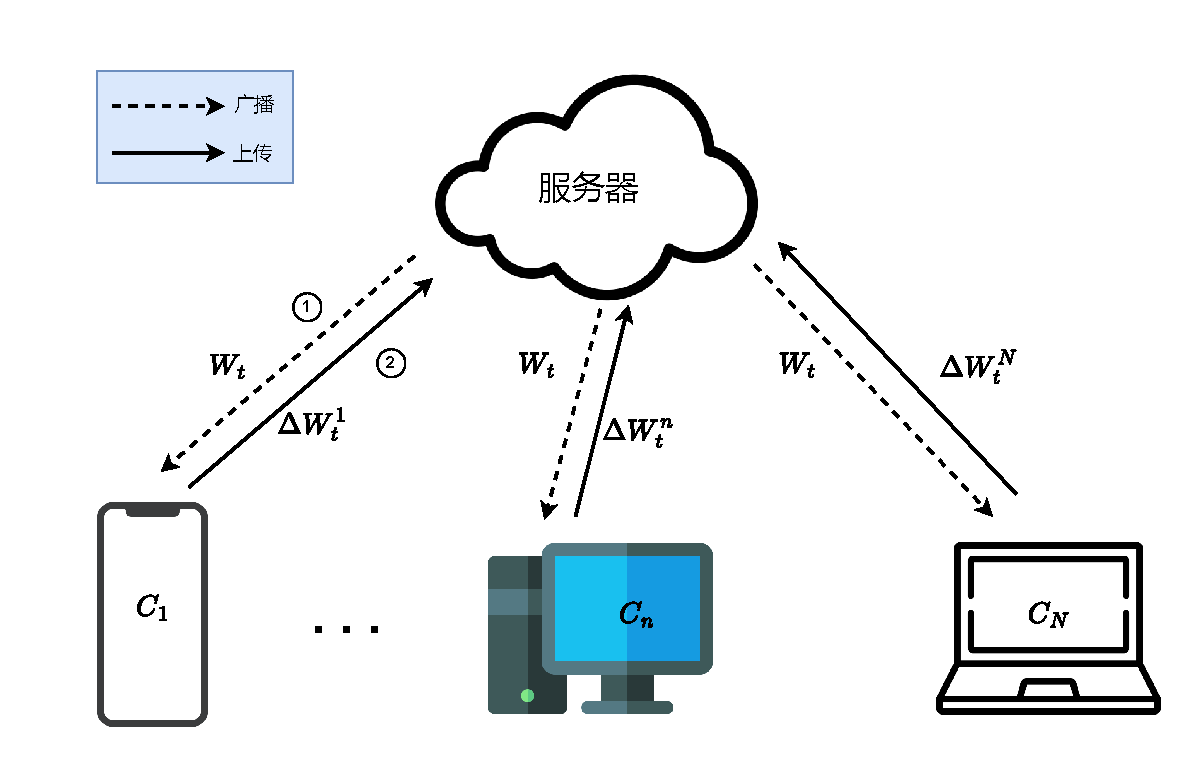
\includegraphics[width=0.9\linewidth]{chapter2/2-1.pdf}
    \caption{\label{fig:2-1}FedAvg算法}
\end{figure}
%ppppppppppppppppppppppppppppppppppppppp

联邦学习算法就是不断重复步骤(1)到步骤(4)重复$T$次,
逐渐最小化下面的公式:
\begin{equation}
    \label{equ:total_fl}
    \underset{\mathbf{w}}{\min} F(\mathbf{w}) = 
    \sum\nolimits_{n \in \mathcal{N}_t} \frac{D_n}{D} F_{n}(\mathbf{w})
\end{equation}
\begin{equation}    
    \label{equ:total_fl_ap}
    F_{n}(\mathbf{w}) = 
    \frac{1}{D_n}\sum_{i=1}^{D_n} f(\mathbf{w};x_n^i,y_n^i)
\end{equation}
其中,$x_n^i$和$y_n^i$表示在边缘设备$n$上的第$i$条数据。
由公式\ref{equ:total_fl}和公式\ref{equ:total_fl_ap}可知,
联邦学习的目标就是找到在多次重复训练上述步骤中使得在选中的边缘设备中
目标损失函数的值最小的模型的参数,
并且可以观察到联邦学习的损失函数是由参与训练的边缘设备的损失函数加权平均
组合而成的损失函数,
边缘设备的损失函数在本地数据集上产生,
这样避免了边缘设备的数据上传到中心侧,
从而极大的保护了边缘设备的数据隐私安全。
公式\ref{equ:total_fl}和公式\ref{equ:total_fl_ap}
是所有联邦学习所优化的目标,
而步骤(1)-(4)是联邦平均算法(FedAvg)的主要过程与相关的参数处理方法。
以下是算法伪代码部分:
%ccccccccccccccccccccccccccccccccccccccccccccccccccccccccccccccc
\begin{algorithm}[H]
    \caption{FedAvg}\label{alg:fedavg}
    \begin{algorithmic}[1]
    \Require 全局模型参数$\mathbf{W}$,
                学习率 $\eta$,
                总通讯次数$T$,
                本地客户端训练次数$E$
    \Ensure $T$轮的全局模型参数$\mathbf{W}_{T+1}$
    \State 初始化全局模型参数$\mathbf{W}_1$
    \Procedure{Server-side Optimization}  {}
        \For {对每个轮次$t \in \{1, \cdots, T \}$}
            \State 随机挑选所有客户端的子集$\mathcal{N}_t$
            \For {对于每个挑选到的客户端$n$并行执行}
                \State $\mathbf{W}_{t+1}^n \leftarrow ClientLocalUpdata(\mathbf{W}_t)$
            \EndFor
            \State 更新全局模型参数
            $\mathbf{W}_{t+1} =
            \sum\nolimits_{n \in \mathcal{N}_t}\frac{D_n}{D}\mathbf{W}_t^n$
        \EndFor
    \EndProcedure

    \Procedure{ClientLocalUpdate}{$\mathbf{W}_t$}
        % \State Receive $\mathbf{w_t^n}$ from the server
        \State 从服务器侧接收$\mathbf{W}_t$
        \State 初始化$\mathbf{w^n_{t,0}} = \mathbf{W}_t$
        % \For{each local iterations $e$ from 1 to $E$}
        \For{从$1$到$E$迭代轮次$e$}
            % \State Update sub-model parameters on private data $\mathbf{w^n_{t,e+1}} = \mathbf{w^n_{t,e}} - \eta \nabla_{\mathbf{w^n_{t,e}}} f_n(\mathbf{w^n_{t,e}})$
            \State 更新本地模型
            $\mathbf{w^n_{t,e+1}} = \mathbf{w^n_{t,e}} - \eta \nabla_{\mathbf{w^n_{t,e}}} f_n(\mathbf{w^n_{t,e}})$
        \EndFor
        \State \Return $\mathbf{w^n_{t,E+1}}$
    \EndProcedure
\end{algorithmic}
\end{algorithm}
%ccccccccccccccccccccccccccccccccccccccccccccccccccccccccccccccc
其中函数Server-side Optimization运行在中心服务器端,
总共运行$T$个轮次,
在每个轮次随机选择跟下一轮次相同比例的客户端执行模型训练,
也即执行ClientLocalUpdata程序,
中心侧服务器端接收客户端程序返回的参数并进行加权聚合。
在客户端侧从服务器端接收当前轮次$t$的全局模型参数,
在本地数据集上对全局模型进行$E$个轮次的训练,
将最终的训练结果上传到服务器端。

\section{卷积神经网络相关知识}
\subsection{深度学习}
深度学习,作为机器学习领域的一个关键分支,采纳了神经网络作为其核心架构,
专注于从图像、语音、文本等多种数据类型中挖掘潜在的规律与特征。
一个典型的深度学习框架,
往往包括了输入层、多个中间隐藏层和输出层。
如图\ref{fig:2-2-1}所示的是一个四层的全连接神经网络,
包括了一个输入层、两个隐藏层和一个输出层,
每个隐藏层包含八个神经元。
% 输入层、输出层以及介于二者之间的多个隐藏层。
与以往需要人工精心设计与提取特征的机器学习方法不同,
深度学习能够直接接纳原始数据作为输入,
并通过多层非线性转换机制,自动提炼出更高层次的特征表示。
这一转变不仅显著提升了特征的质量,还极大地减轻了人工操作的负担。
此外,在多个应用领域内,深度学习技术已经展现出了超越传统机器学习方法的卓越性能。
它凭借海量的数据与强大的计算能力,
能够训练出极为复杂的模型,从而灵活应对各种复杂多变的实际应用场景。
%ppppppppppppppppppppppppppppppppppppppp
\begin{figure}[H]
    \centering
    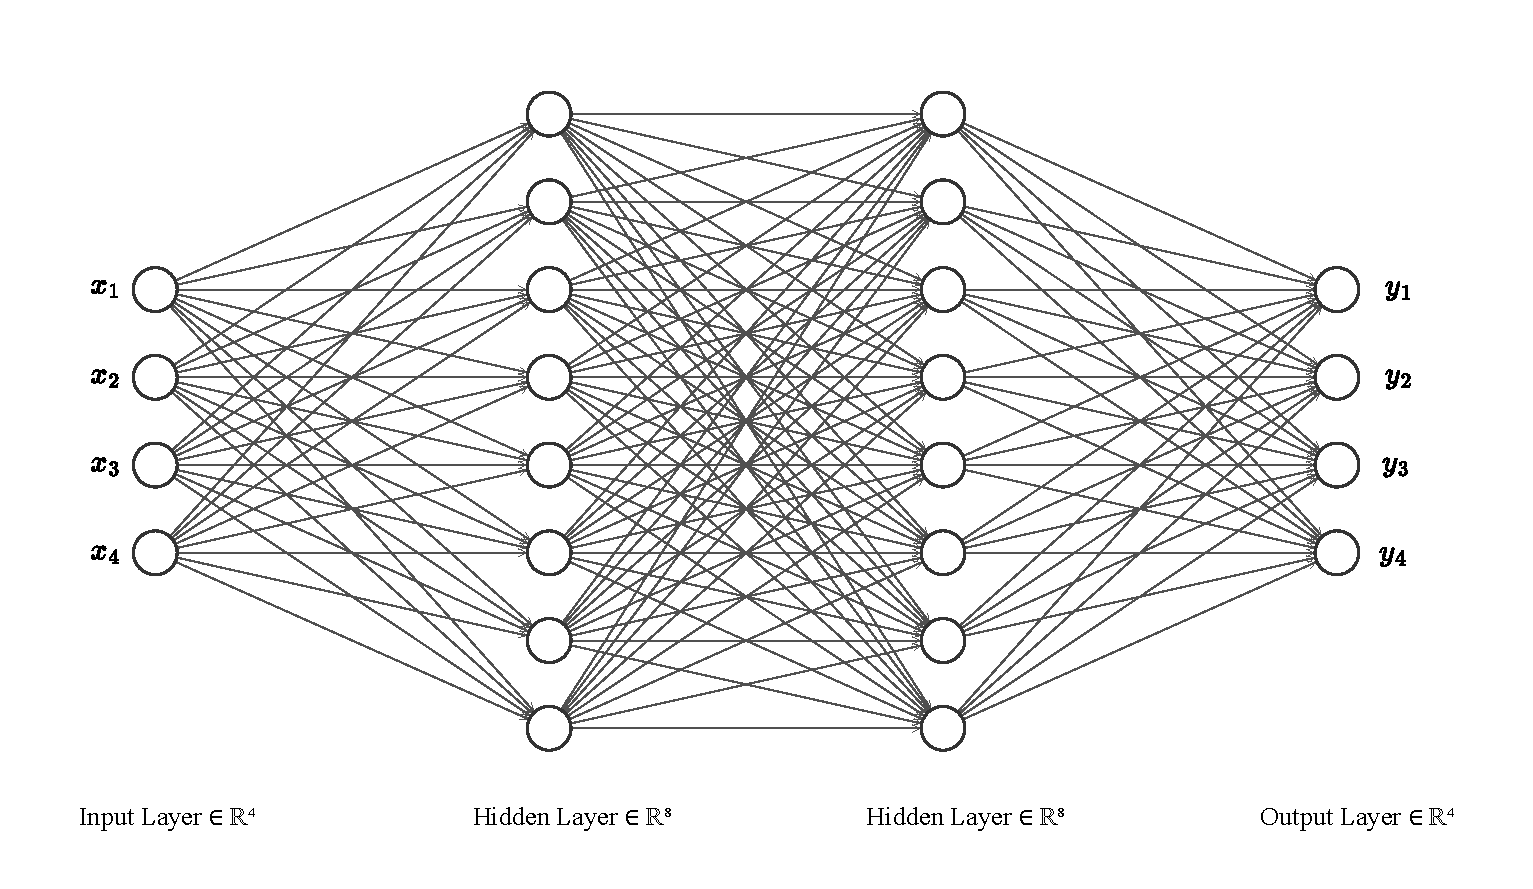
\includegraphics[width=0.9\linewidth]{chapter2/2-2-1深度学习.pdf}
    \caption{\label{fig:2-2-1}深度学习四层全连接神经网络}
\end{figure}
%ppppppppppppppppppppppppppppppppppppppp
在图\ref{fig:2-2-1}中可以看到全连接神经网络中每层都包含一定数量的神经元,
每个神经元代表一个值。
除了输入层与输出层之外的每一个中间隐藏层都与上层下层神经元存在联系。
详细的结构如图\ref{fig:2-2-1-neuron}所示,
对上层的每个神经元做加权求和,
在加上上层的偏差值,
图中上层共有四个神经元与四个加权参数和一个偏差值$b$,
最后经过非线性映射输出下一个神经元,
非线性映射通过激活函数来实现,
常用的有ReLU之类的,
最后输出图中的下层神经元$y$。
%ppppppppppppppppppppppppppppppppppppppp
\begin{figure}[H]
    \centering
    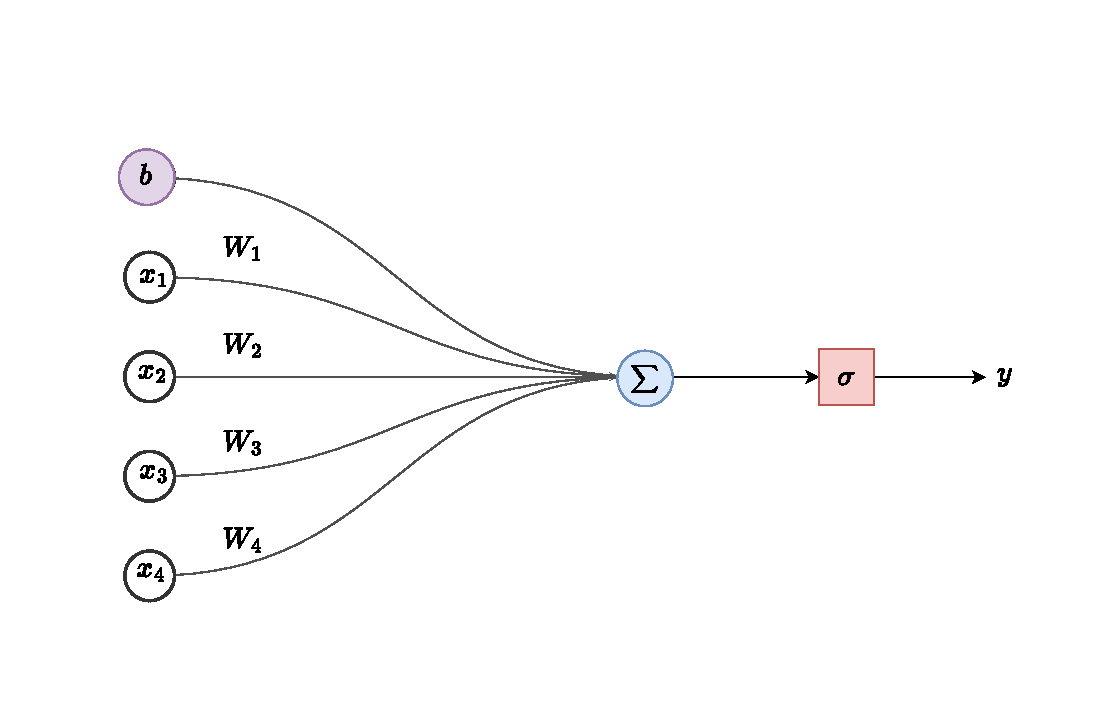
\includegraphics[width=0.9\linewidth]{chapter2/2-2-1神经元.pdf}
    \caption{\label{fig:2-2-1-neuron}全连接神经元结构图}
\end{figure}
%ppppppppppppppppppppppppppppppppppppppp
上述描述了深度学习神经网络的前向传播过程,
前向传播对神经元需要学习的东西进行了预测。
而在训练过程中主要使用反向传播算法\cite{lecun1989backpropagation}
(BackPropagation,BP)进行训练,
反向传播通过随机梯度下降的方法减小前向传播预测的标签与真是标签的误差,
主要实现方式是不断修正神经网络中的权重与偏差来最小化优化目标。

\subsection{卷积神经网络}
卷积神经网络(Convolutional Neural Networks, CNNs)
是一种专门用于处理数据有网格结构的深度学习模型,
最早在图像识别和处理任务中取得了显著的效果。
CNN的核心是卷积层和池化层的堆叠,
通过这些层提取图像的空间和位置特征。
与传统的全连接网络不同,
CNN使用局部连接和权重共享,
使其在处理高维图像数据时具有较少的参数、更低的计算成本,
同时保持了强大的特征提取能力。
%ppppppppppppppppppppppppppppppppppppppp
\begin{figure}[H]
    \centering
    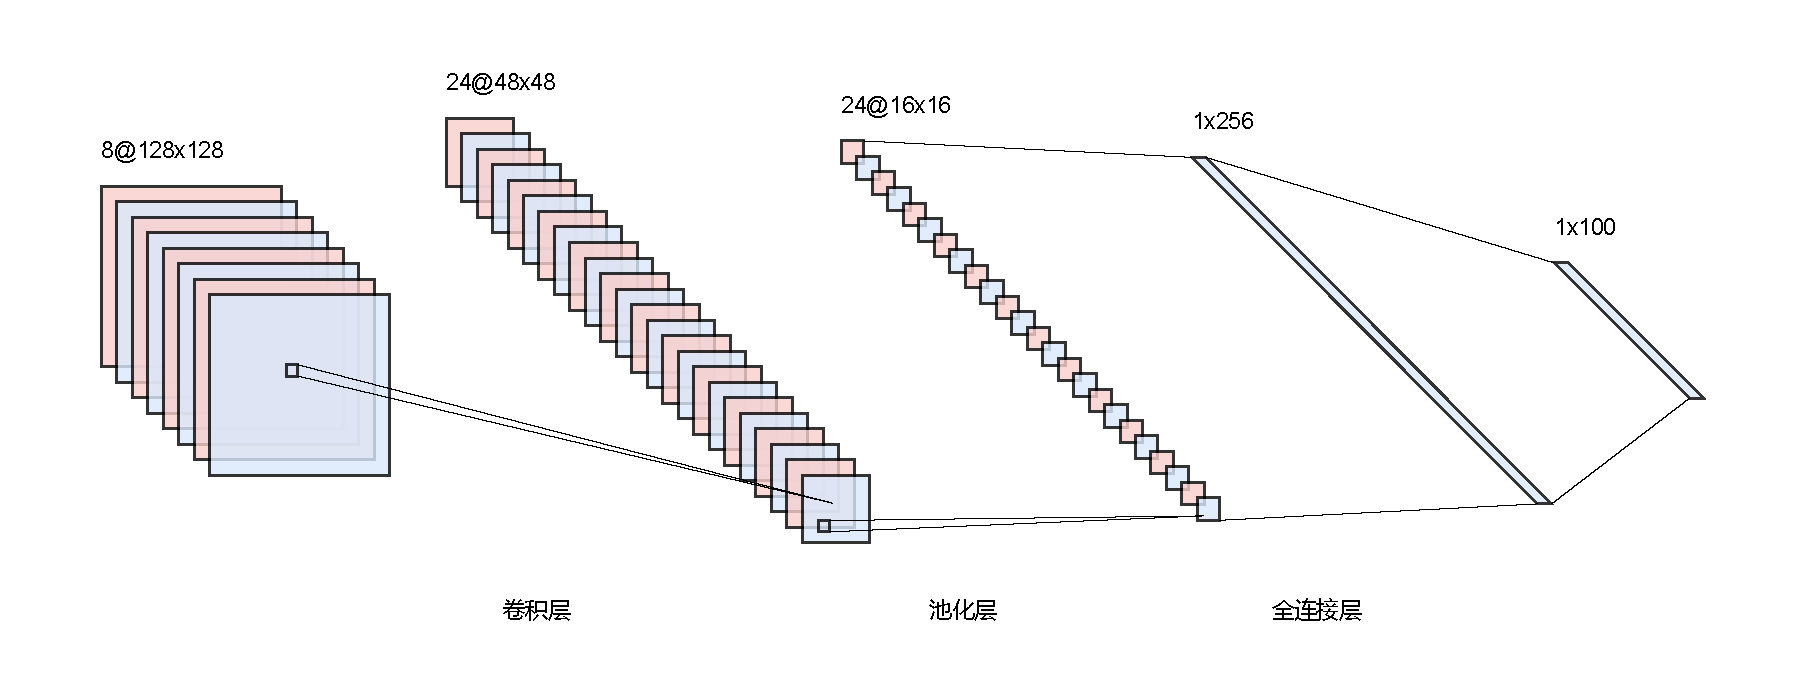
\includegraphics[width=0.9\linewidth]{chapter2/2-2-2卷积神经网络.pdf}
    \caption{\label{fig:2-2-2-conv}卷积神经网络示意图}
\end{figure}
%ppppppppppppppppppppppppppppppppppppppp
如图\ref{fig:2-2-2-conv}所示,
卷积神经网络主要包括输入层、卷积层、池化层、激活层、全连接层以及输出层构成。
输入的特征信息主要有卷积层和池化层主要用来提取特征信息,
这些层在整个卷积神经网络中可以不断的有规律的堆叠,
全连接层以及输出层根据任务的不同输出不同的信息,
主要针对任务做出改变。
下面将详细介绍卷积神经网络的各个主要模块:

(1)卷积层

卷积层(Convolutional Layer)是卷积神经网络的核心组件,
其作用是提取输入数据的局部特征。
卷积层的运作基于卷积运算,通过多个卷积核(filter)
滑动窗口来扫描输入数据的不同区域,从而提取数据的局部信息,
比如边缘、纹理和形状等特征。
卷积层一般有卷积核、步幅(Stride)以及填充(Padding)等参数。
卷积核,也称为滤波器,是一个小的矩阵(通常为3x3、5x5等),
其中的参数是可以训练的权重。
卷积核在输入数据上逐点滑动(即做卷积操作),
通过对局部区域进行加权求和得到特征映射。不同的卷积核会提取不同的特征,
比如边缘、颜色变化、纹理等。
步幅决定了卷积核在输入数据上每次移动的步长。
填充是指在输入数据的边缘添加额外的像素,使得卷积核在边缘位置时也能充分计算。
积操作生成的输出结果称为特征图,它展示了卷积核在整个输入数据上的响应。
特征图的大小由卷积核大小、步幅、填充方式共同决定。

卷积核的参数在整个输入上共享,显著减少了网络的参数量,提升了训练效率。
而且卷积核只连接局部区域,减少了计算量,同时有助于模型专注于图像的局部特征。
卷积操作使得特征对平移有一定不变性,提升了模型对输入变化的鲁棒性。
卷积层能够有效地提取数据中的空间特征,通过多个层级的卷积操作,
网络可以逐步抽象出更高层次的特征。

(2)池化层

池化层(Pooling Layer)是卷积神经网络中的一个重要组件,
其主要作用是对特征图进行下采样,
从而减小特征图的尺寸和参数量,缓解过拟合,
提高计算效率,同时保持主要特征信息。
池化层通过聚合局部区域的特征,帮助模型在识别物体特征时获得平移不变性。
池化层会减小输入特征图的空间维度(宽度和高度),
从而减少后续层的计算和内存需求。
例如,如果输入图像大小为64×64,
通过一次2x2池化操作可以将其尺寸缩减为 
32×32,大大减少后续层的计算量。
并且池化操作通过减少特征图的尺寸,减小了模型的自由度,
从而降低了过拟合的风险。
在特征图降维的同时,它还保留了数据的主要信息,
确保模型仍能有效学习输入数据的主要特征。
池化层还有助于增强模型对输入数据的平移不变性,即使输入图像发生小幅移动或变形,
池化后的特征图依然能很好地描述这些信息。

池化层一般有三种池化方式,
\textbf{最大池化(Max Pooling)}、
\textbf{平均池化(Average Pooling)}
以及\textbf{全局平均池化}\cite{lin2013network}\textbf{(Global Average Pooling)}。
最大池化是最常见的池化操作,它在池化窗口内取最大值,保留最显著的特征。
最大池化常用于提取图像的边缘或亮度等重要信息,忽略细微的变化。
平均池化是在池化窗口内取平均值,将窗口内的数值平均化。
这种方法会更平滑地表示特征图的变化,通常用于减少数据的噪声。
全局平均池化(Global Average Pooling, GAP)会在整个特征图上计算平均值,
即每个通道只有一个数值。
GAP常用于分类任务中的最后一层,将每个通道的信息汇总为一个数值,
用于全连接层或分类输出。

(3)全连接层

全连接层(Fully Connected Layer, FC Layer)是神经网络中的一种关键层,
通常用于将特征向量转换为分类、回归或其他形式的输出。
在全连接层中,每个输入节点和输出节点之间都有连接,因此称为“全连接”。
全连接层通常位于网络的末端,它接收来自卷积层或池化层的高层次特征并进行整合,
用于最终的决策输出。
全连接网络的核心是矩阵运算,具体运算公式是\ref{equ:fclayer},
在上一小章节详细的介绍了全连接神经网络的具体细节。
\begin{equation}
    \label{equ:fclayer}
    Y = W \cdot X + b
\end{equation}

(4)激活函数

激活函数\cite{sharma2017activation}(Activation Function)是神经网络中的关键组件,
它的作用是引入非线性,使得神经网络能够拟合复杂的非线性关系。
若没有激活函数,神经网络只能表示线性映射,无法有效解决复杂的分类或回归问题。
激活函数通常位于每一层神经元的输出之后,接受线性组合的输入并进行非线性变换,
输出结果用于下一层的计算。
常见的激活函数有Sigmoid、Tanh、ReLU、Swish等等,下面将详细介绍这些激活函数。
%ppppppppppppppppppppppppppppppppppppppp
\begin{figure}[H]
    \centering
    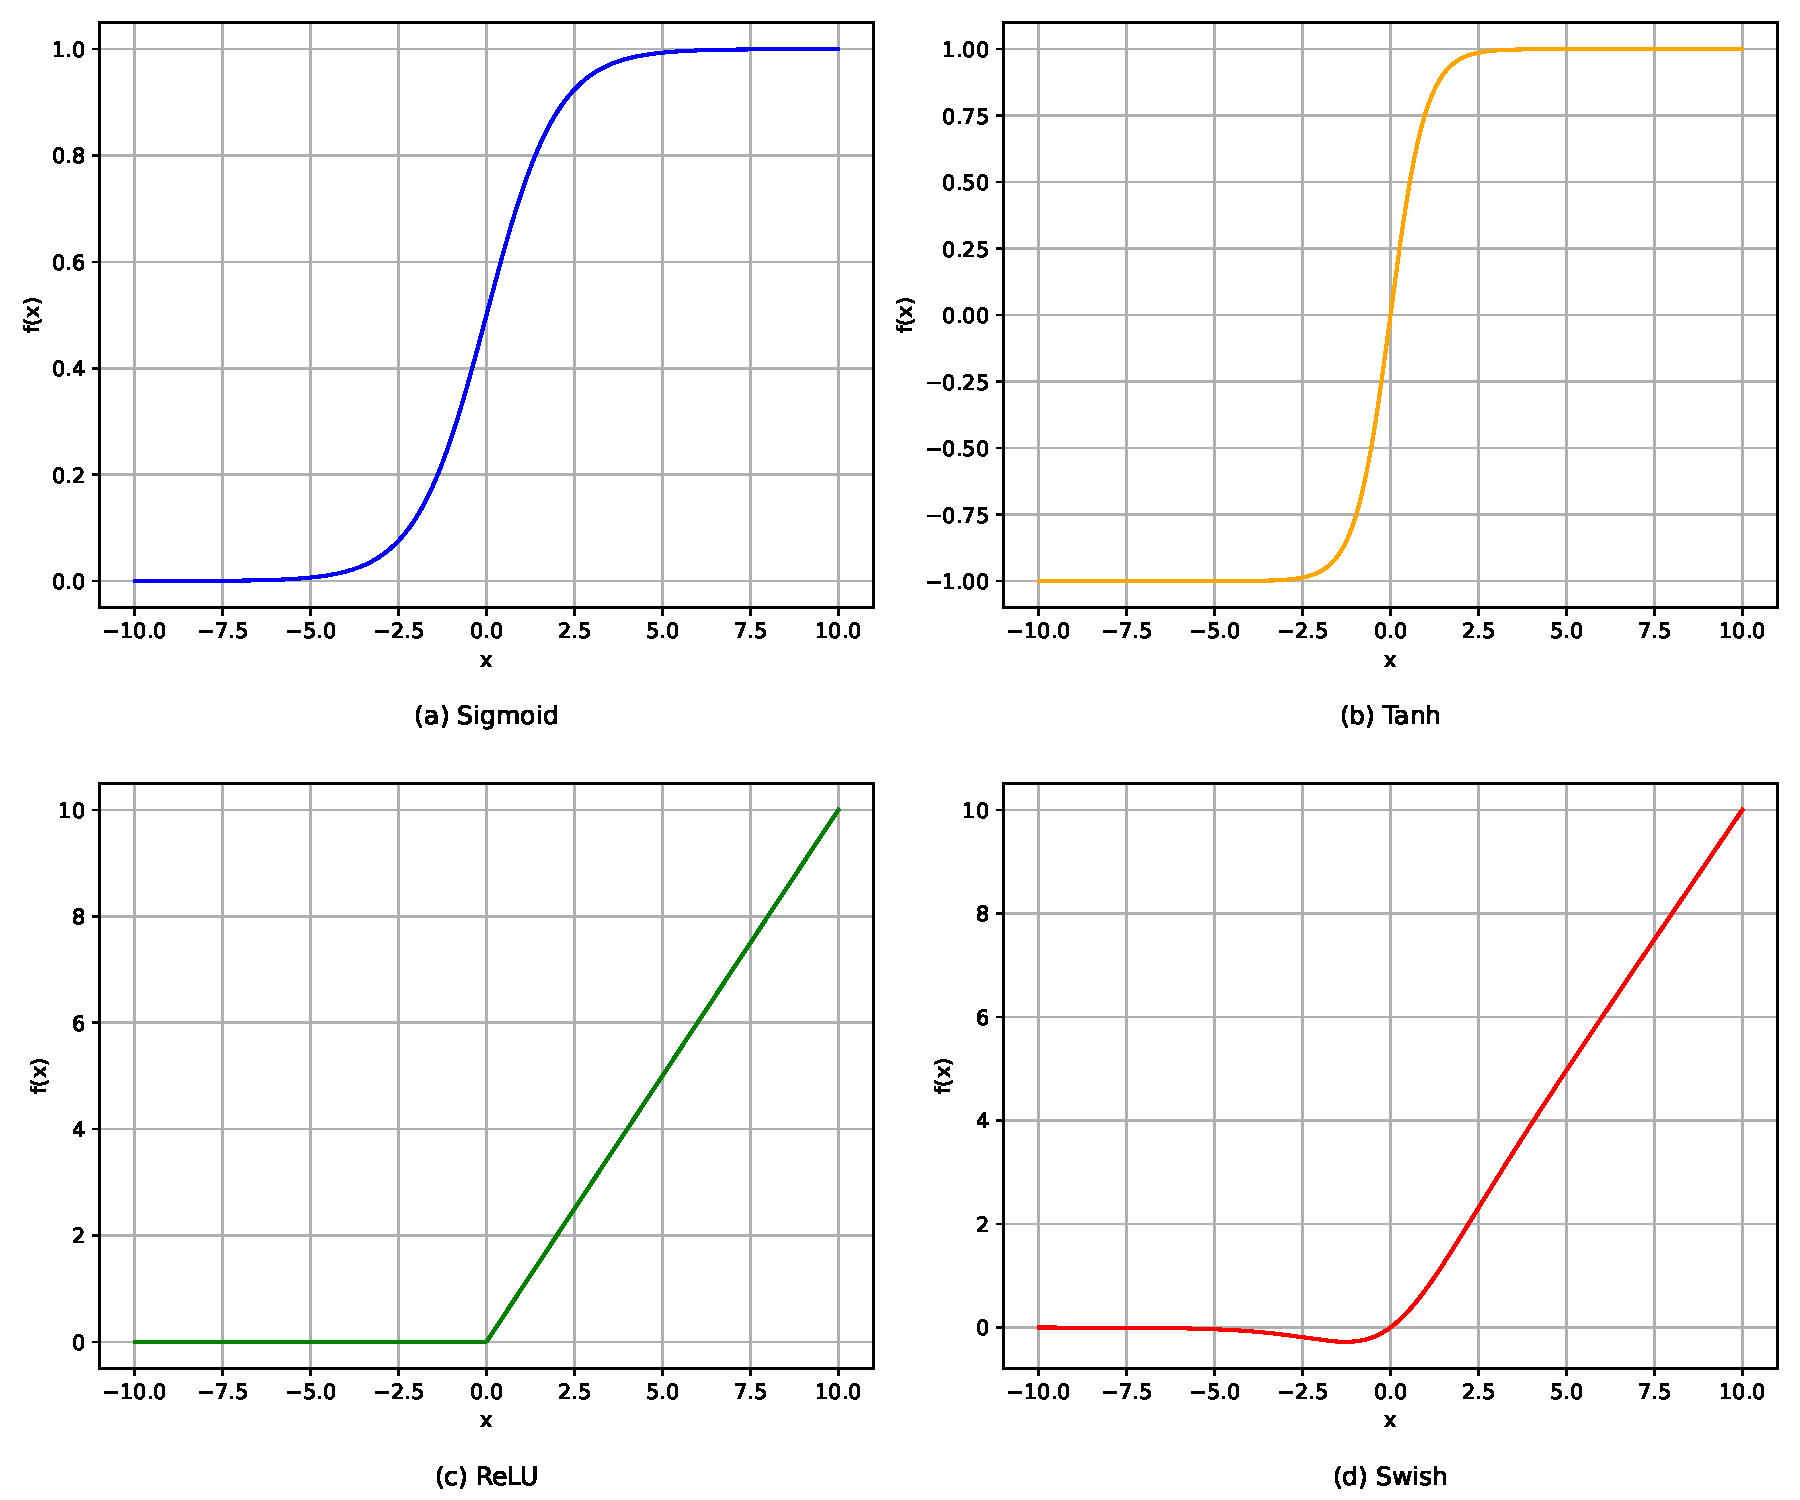
\includegraphics[width=0.9\linewidth]{chapter2/activation_functions.pdf}
    \caption{\label{fig:2-2-2-activate_fc}四种常用的激活函数}
\end{figure}
%ppppppppppppppppppppppppppppppppppppppp
Sigmoid函数将输入映射到 (0,1) 区间,适合概率输出(如二分类任务)。
早期广泛应用,但较少用于深层网络,因为容易导致梯度消失问题,
尤其是在深层网络中,导致学习过程缓慢。
较为明显的是Sigmoid 函数的梯度在接近 0 或 1 时趋近于 0,导致梯度消失。
并且Sigmoid 函数输出是非对称的,可能导致反向传播时梯度更新不稳定。
其图像可见图\ref{fig:2-2-2-activate_fc}(a)所示,
下面是Sigmoid函数的公式:
\begin{equation}
    f(x) = \sigma (x) = \frac{1}{1+e^{-x}}
\end{equation}

Tanh函数将输入映射到 (−1,1) 区间,且输出是零中心的,有利于梯度更新。
相较于 Sigmoid,Tanh 函数可以减少梯度消失问题,但在深层网络中仍然可能出现梯度衰减。
对于较大的输入,Tanh 的梯度也趋近于 0,导致梯度消失。
其图像可见图\ref{fig:2-2-2-activate_fc}(b)所示,
下面是Tanh函数的公式:
\begin{equation}
    f(x) = \tanh(x) = \frac{e^x-e^{-x}}{e^x+e^{-x}}
\end{equation}

ReLU 函数(Rectified Linear Unit)输出范围$[0,+\infty]$,
将负数部分直接设为0,保持正数部分不变,具有稀疏激活的特点(即部分神经元被激活)。
计算简单、高效,梯度在正区间不会衰减,因此常用于深层网络中,显著加速训练过程。
但是当神经元的输入为负时,ReLU 的梯度为0,
神经元无法更新,可能导致一部分神经元“死亡”。
其图像可见图\ref{fig:2-2-2-activate_fc}(c)所示,
下面是ReLU函数的公式:
\begin{equation}
    f(x)=\max(x, 0)
\end{equation}

Swish函数是由 Google 提出的,结合了ReLU和Sigmoid的特性,
既包含非线性又不会像ReLU那样直接截断。
Swish 的输出不再严格限制为正值,且对于小的负输入也有较小的梯度,
适合深层网络,可以带来更好的训练效果。
其图像可见图\ref{fig:2-2-2-activate_fc}(d)所示,
下面是Swish函数的公式:
\begin{equation}
    f(x)= \sigma (x) \cdot x =\frac{x}{1+e^{-x}}
\end{equation}
除此之外, maxout\cite{goodfellow2013maxout}、 
ELU\cite{clevert2015fast}等激活函
数也有着广泛的使用。


\subsection{卷积神经网络模型}
本章介绍本论文算法所使用的卷积神经网络模型,分别是简单的多层卷积神经网络
与ResNet系列的ResNet18与ResNet34。
下面分别详细的介绍本文用到模型的架构。

(1)四层CNN模型

如图\ref{fig:2-2-3-simplecnn}所示,
本文所用的cnn模型由4个块加上一个全连接层组成,
每个块先经过一个卷积层对上层传来的特征图进行特征提取,
随后对提取到的特征图做标准化处理,
标准化处理之后经过ReLU激活函数,
在块的最后一层是池化层。
四层块中的卷积层是不同尺寸的卷积核。
图片从经过四块之后,
最后经过全连接层,全连接层根据分类任务的类别数,
改变全连接层最后的输出数,
本文中用到十分类。
%ppppppppppppppppppppppppppppppppppppppp
\begin{figure}[H]
    \centering
    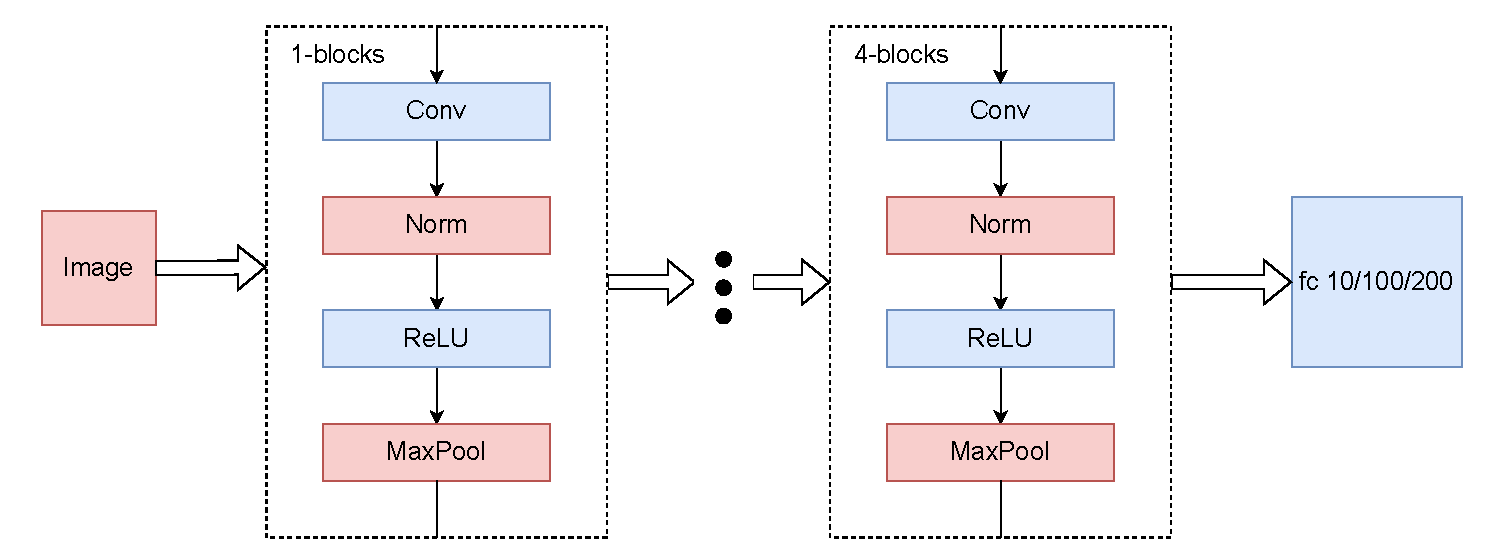
\includegraphics[width=1 \linewidth]{chapter2/simple_cnn.pdf}
    \caption{\label{fig:2-2-3-simplecnn}简单CNN模型架构}
\end{figure}
%ppppppppppppppppppppppppppppppppppppppp
(2)ResNet系列模型

ResNet(Residual Network)系列模型是由微软研究院提出的一种深度神经网络架构,
主要应用于图像识别和分类任务。
\begin{table}[h!]
    \centering
    \caption{\label{tab:resnet}ResNet系列模型详细信息}
    \begin{tabularx}{\linewidth}{c|X<{\centering}|X<{\centering}|X<{\centering}}
    \hline
    \textbf{layer name} & \textbf{output size} & \textbf{18-layer} & \textbf{34-layer}  \\ \hline
    conv1 & 112$\times$112 & \multicolumn{2}{c}{7$\times$7, 64, stride 2} \\ \hline
    \multirow{2}{*}{\makecell[c]{conv2\_x}} & \multirow{2}{*}{\makecell[c]{56$\times$56}} & \multicolumn{2}{c}{3$\times$3 max pool, stride 2} \\ \cline{3-4}
     &  & \(\begin{bmatrix} 3 \times 3, 64 \\ 3 \times 3, 64 \end{bmatrix} \times 2\) &   \(\begin{bmatrix} 3 \times 3, 64 \\ 3 \times 3, 64 \end{bmatrix} \times 3\) \\ \hline
    conv3\_x & 28$\times$28 & \(\begin{bmatrix} 3 \times 3, 128 \\ 3 \times 3, 128 \end{bmatrix} \times 2\) &  \(\begin{bmatrix} 3 \times 3, 128 \\ 3 \times 3, 128 \end{bmatrix} \times 4\) \\ \hline
    conv4\_x & 14$\times$14 & \(\begin{bmatrix} 3 \times 3, 256 \\ 3 \times 3, 256 \end{bmatrix} \times 2\) &  \(\begin{bmatrix} 3 \times 3, 256 \\ 3 \times 3, 256 \end{bmatrix} \times 6\) \\ \hline
    conv5\_x & 7$\times$7 & \(\begin{bmatrix} 3 \times 3, 512 \\ 3 \times 3, 512 \end{bmatrix} \times 2\) &  \(\begin{bmatrix} 3 \times 3, 512 \\ 3 \times 3, 512 \end{bmatrix} \times 3\) \\ \hline
    &1$\times$1 & \multicolumn{2}{c}{average pool, 1000-d fc, softmax} \\ \hline
    \multicolumn{2}{c|}{FLOPs} & $1.8\times10^9$ & $3.6\times10^9$  \\ \hline
    \end{tabularx}
\end{table}
ResNet的核心思想是引入残差连接(Residual Connection),即跳跃连接,
用于解决深层神经网络中的梯度消失和模型退化问题。
随着ResNet模型层数的增加,它依旧能保持较好的性能,
甚至在更深的网络中取得了更高的准确率。下面是对ResNet系列模型的详细介绍。

在普通的深层神经网络中,随着层数增加,梯度可能会逐渐变小,
从而使得模型很难学习深层特征。
而ResNet通过残差连接的设计,使得信息能够直接从前层传递到后层,
帮助梯度更容易地传递,避免了梯度消失问题。
残差块(Residual Block)是ResNet的基本单元。其核心公式为:
\begin{equation}
    \mathbf{y} = \mathsf{F}(\mathbf{x}) + \mathbf{x}
\end{equation}
如图\ref{fig:2-2-2-resnet}所示,
输入$\mathbf{x}$在经过Conv1层个ReLU之后再经过Conv2层,
在下一个ReLU层之前两者的输出相加和,
之后经过最后一层输出到下一个块。
在最后一块之后是一个全连接层,
根据自己所需要分类的类别设置输出的数量,
例如在CIFAR10上就设定为10。
%ppppppppppppppppppppppppppppppppppppppp
\begin{figure}[H]
    \centering
    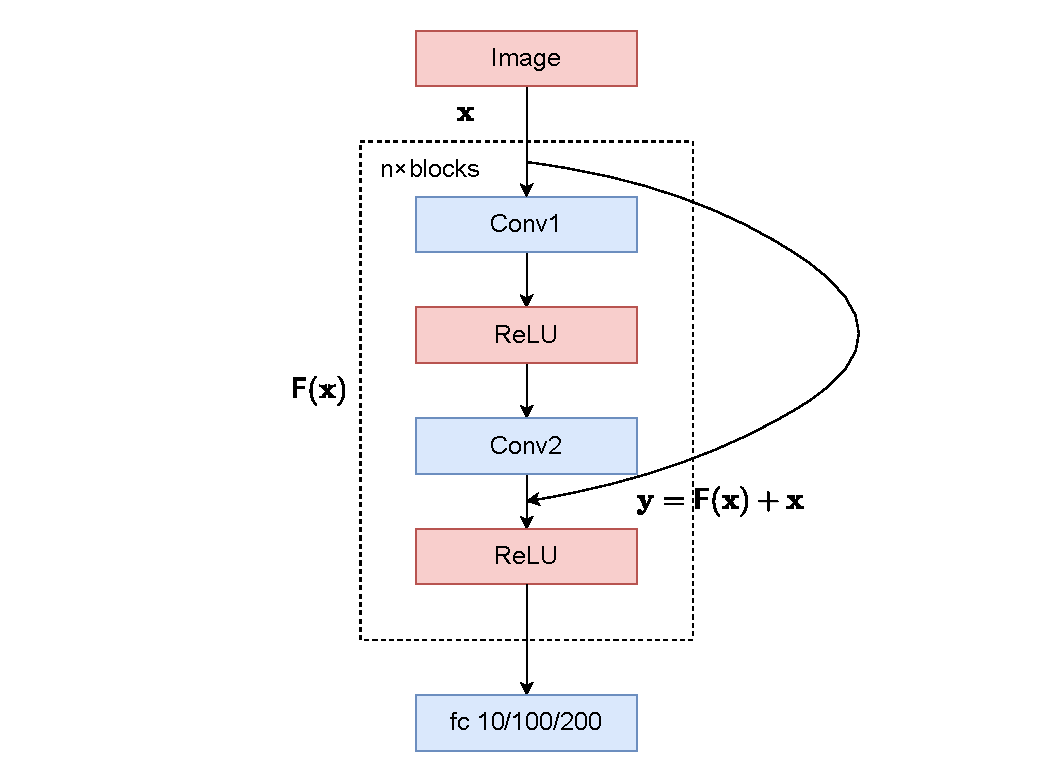
\includegraphics[width=0.9\linewidth]{chapter2/resnet.pdf}
    \caption{\label{fig:2-2-2-resnet}残差结构示意图}
\end{figure}
%ppppppppppppppppppppppppppppppppppppppp

ResNet18和ResNet34的具体结构如表\ref{tab:resnet}所示,
都是五层结构,
除了第一个块的卷积核是$7 \times 7$之外,
其余的卷积核都是$3 \times 3$。
ResNet18和ResNet34的不同之处就是每块中的相同的卷积层堆叠层数不同。

% \section{蒸馏学习相关知识}
% 在介绍蒸馏学习之前,先介绍一下\textbf{KL散度}的概念。
% KL散度(Kullback-Leibler Divergence,简称KL Divergence),
% 也称为相对熵,是信息论中衡量两个概率分布之间差异的一种方法。
% 它表示一个分布$Q$相对于另一个分布$P$的信息损失,
% 常用于机器学习、深度学习以及自然语言处理等领域。
% 在蒸馏学习中用于衡量软标签与学生模型的分布差距损失。
% KL散度的数学定义为:
% \begin{equation}
%     D_{KL}(P \| Q) = \int P(x) \log  \frac{P(x)}{Q(x)} dx
% \end{equation}
% 其中$P(x)$是真实分布,
% $Q(x)$是近似分布。
% KL散度可以理解为, 
% 如果事件实际分布为$P$,
% 而我们使用$Q$来描述这些事件,
% 那么KL散度衡量的是因错误使用$Q$分布而多花费的信息量(以比特或自然对数单位表示)。

% 知识蒸馏(Knowledge Distillation)是一种在深度学习中常用的模型压缩和加速方法,
% ,旨在将大规模、复杂的“教师模型”(Teacher Model)中学到的知识转移到
% 一个较小的“学生模型”(Student Model)中,
% 从而在不显著损失性能的情况下,
% 降低模型的计算复杂度并减小模型大小。
% 知识蒸馏最早由Hinton等人在2015年提出,
% 通过“软标签”(Soft Targets)和“硬标签”(Hard Targets)的组合训练学生模型,
% 从而实现信息迁移。
% %ppppppppppppppppppppppppppppppppppppppp
% \begin{figure}[H]
%     \centering
%     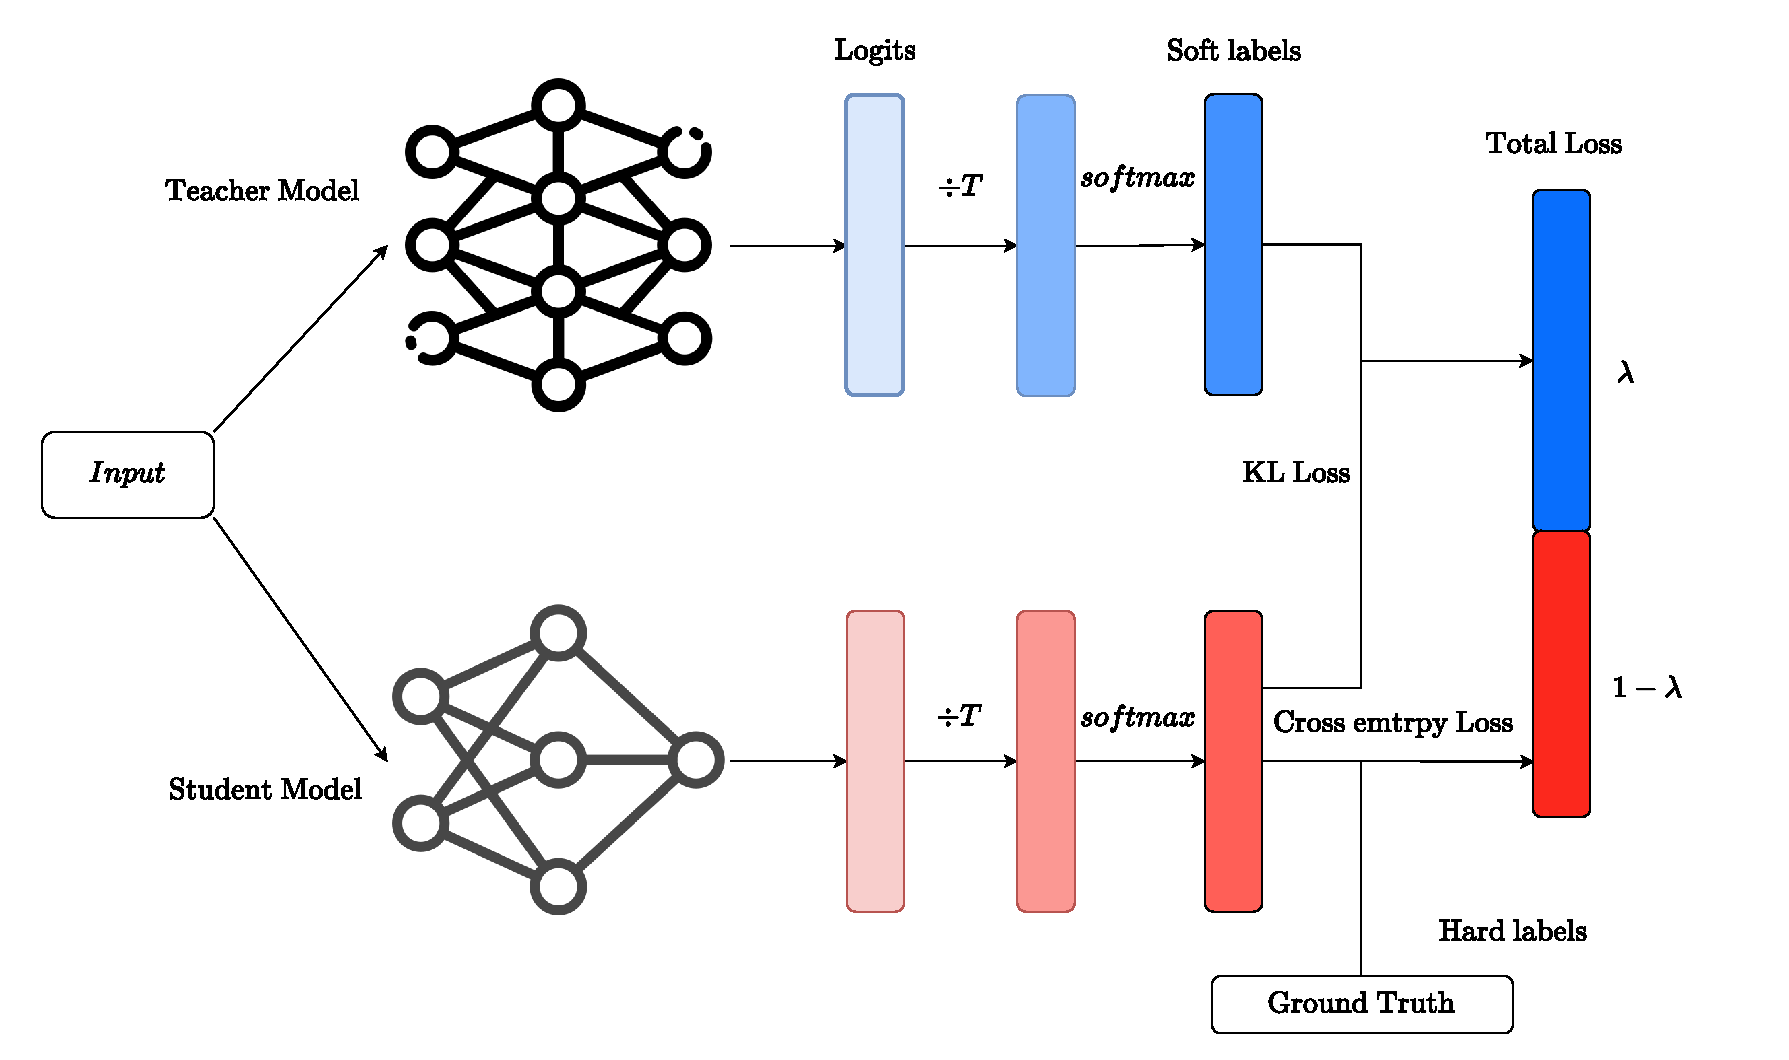
\includegraphics[width=0.9\linewidth]{chapter2/2-3蒸馏学习.pdf}
%     \caption{\label{fig:2-3kllearn}蒸馏学习示意图}
% \end{figure}
% %ppppppppppppppppppppppppppppppppppppppp

% 在知识蒸馏过程中,教师模型的输出通常不只是最终的预测标签(硬标签),
% 而是包含了类别概率分布的软标签,这种概率分布反映了教师模型对各类的信任程度。
% 通过软标签信息,学生模型可以学习到更丰富的类别间关系。
% 知识蒸馏的主要流程如图\ref{fig:2-3kllearn}所示:
% \textbf{教师模型训练}:
% 首先训练一个性能优异、规模较大的教师模型,通常为深层神经网络模型,
% 如大型卷积神经网络或预训练的大型语言模型。
% \textbf{蒸馏过程}:
% 在训练学生模型时,加入教师模型的预测作为监督信号。
% 具体而言,学生模型不仅学习数据集的真实标签,
% 还学习教师模型输出的软标签(通常经过温度调节,以平滑概率分布),
% 以便更好地复现教师模型的知识。
% \textbf{学生模型训练}:
% 通过联合优化真实标签的交叉熵损失和软标签的蒸馏损失(使用KL散度计算),
% 使学生模型在保持高准确率的同时具备更高的推理效率。

% 知识蒸馏的优点在于能够在保留模型性能的前提下显著减少模型参数量和推理时间,
% 因此被广泛应用于边缘计算和移动设备等计算资源受限的场景中。
% 此外,知识蒸馏还被用于模型集成,通过多个教师模型的知识整合,
% 进一步提升学生模型的表现。
% 按照蒸馏方式可以分为三种:

% (1)离线蒸馏(Offline Distillation)

% 离线蒸馏是知识蒸馏最经典的一种形式,也是最常用的方式。
% 在这种方法中,教师模型和学生模型的训练过程是分离的。
% 教师模型通常是一个预先训练好且性能优异的大型模型,
% 已完全冻结,不会在蒸馏过程中更新,
% 学生模型通过学习教师模型生成的软标签和真实标签联合优化其参数,
% 教师模型和学生模型的训练过程相互独立。
% 离线蒸馏多用于模型压缩,例如用大规模预训练模型指导轻量级模型的训练。


% (2)在线蒸馏(Online Distillation)

% 在线蒸馏是一种教师模型和学生模型同时训练的知识蒸馏方法。
% 在这种方式中,教师模型的知识随着训练过程动态更新。
% 教师模型在训练过程中实时更新,不是一个静态的模型,
% 可以采用多个学生模型互为教师的方式(即无明确教师模型),
% 与离线蒸馏相比,在线蒸馏不需要分阶段训练。
% 在线蒸馏通常用于深度模型的动态优化场景,例如自动驾驶、实时推理系统等。

% (3)自蒸馏(Self-Distillation)

% 自蒸馏是一种特殊的知识蒸馏方法,其中没有明确的教师模型,
% 学生模型通过自身的不同输出层或训练阶段提供知识指导。
% 学生模型通过自身的结构学习更深层次的知识,
% 例如利用较深层次的输出指导浅层的训练。
% 通过分阶段训练,不断将前一阶段的模型作为下一阶段的“教师”。
% 自蒸馏被广泛用于模型优化,如深度网络内部层次的自监督学习或小模型自我增强。

\section{本章小结}
本章首先介绍了联邦学习的经典框架以及联邦学习需要优化的目标
并给出了联邦学习中经典算法FedAvg的伪代码实现。
其次介绍了可以应用到联邦学习框架的深度学习模型,
详细的介绍了计算机视觉中用到的卷积层、全连接层、激活函数等等
需要用到的基础知识,
其中着重介绍了本论文需要用的模型,
分别是简单的四层卷积神经网络和ResNet系列模型的基础架构模型内部细节。
% 最后介绍了蒸馏学习的相关知识。